\documentclass{sig-alternate}

\usepackage{algorithmic}
\usepackage{algorithm}

\begin{document}

\conferenceinfo{WSDM}{'11 Hong Kong}
%\CopyrightYear{2007} % Allows default copyright year (20XX) to be over-ridden - IF NEED BE.
%\crdata{0-12345-67-8/90/01}  % Allows default copyright data (0-89791-88-6/97/05) to be over-ridden - IF NEED BE.

%\title{A Novel Approach to Profile Based Personalized Web Search and its Evaluation}%\titlenote{(Produces the
\title{Personalizing Web Search Using Long Term Browsing History}

\numberofauthors{3}

\author{
\alignauthor
Nicolaas Matthijs\\
       \affaddr{University of Cambridge}\\
       \affaddr{15 JJ Thomson Avenue}\\
       \affaddr{Cambridge CB3 0FD, UK}\\
       \email{nm417@cam.ac.uk}
% 2nd. author
\alignauthor
Filip Radlinski\\
       \affaddr{Microsoft Research}\\
       \affaddr{7 J J Thomson Ave}\\
       \affaddr{Cambridge CB3 0FB, UK}\\
       \email{filiprad@microsoft.com}
% 3rd. author
\alignauthor Stephen Clark\\
       \affaddr{University of Cambridge}\\
       \affaddr{15 JJ Thomson Avenue}\\
       \affaddr{Cambridge CB3 0FD, UK}\\
       \email{sc609@cam.ac.uk}
}

%Given the abundance of information available on the World Wide Web, personalized search is a potential way in which search results can be improved for the wide range of users with different information needs out there, and some personalized search strategies have already been successfully deployed. However, a lot of these rely on very shallow user and user behavior modeling. In this paper, we study various algorithms that use a person's complete browsing history as input data. Using the specific characteristics of the web and more advanced NLP techniques, we attempt to implicitly learn a user's interests and generate an interest profile. We are the first ones to successfully deploy a combination of user profile and click based methods for re-ranking search engine results in order to make them more biased towards the current user's personal interest. Our evaluation framework suggests a method in which personalized search can be evaluated in a more reliable and thorough way. One of the main goals of the paper was to develop a method and tool that is directly useful and applicable to real users, and can be downloaded and used in the form of a Firefox add-on. Therefore, performance and usability issues had to be taken into account as well. In doing this, we still succeeded in obtaining results that are significantly better than the default search engine ranking or previously suggested personalized search strategies.

\maketitle
\begin{abstract}
In this paper, we study various algorithms that use a person's complete browsing history as input data for web search personalization. Using the specific characteristics of the web and more advanced NLP techniques, we attempt to implicitly learn a user's interests and generate an interest profile.  We develop an end to end search personalization system, being the first to give a detailed evaluation with both offline and online experiments. One of the additional goals of the paper was to develop a scalable and user-friendly tool that is directly useful and applicable to end users, and can be downloaded and used as a Firefox add-on. In doing this, we succeeded in obtaining results that are significantly better than the default search engine ranking or previously published personalized search strategies.
\end{abstract}

\category{H.3.3}{Information Storage and Retrieval}{Information Search and Retrieval}

\terms{Algorithms, Experimentation, Measurement}

\keywords{AlterEgo, Browsing History, Evaluation, Personalized Web Search, Interleaving, Searching, Ranking, User Profile}

\section{Introduction}
Although information retrieval systems such as web search have become an essential part of our lives, there is still room for improvement. A major deficiency of current retrieval systems is that they are not adaptive enough to a user's individual needs and interests \cite{Teevan:Potential}. This can be illustrated with the search query ``ajax". This query will return results about Ajax based web development, about the Dutch football team Ajax Amsterdam and websites about the cleanser named Ajax. Meanwhile, different users would clearly prefer different results. Without personalization, however, all users will be presented with the same ranking.

Additionally, previous research has noted that the vast majority of search queries are short \cite{Silverstein:Marais, Jansen:Spink} and ambiguous \cite{Cronen:Townsend, Sanderson:Mark}. Often, different users will use the same query to express a completely different information need  \cite{Teevan:Potential, Jansen:Spink, Qiu:Cho, Shen:Tan, Teevan:Value}. Personalized search is a potential solution to this problem.

A large range of personalization strategies have previously been suggested, including \cite{Teevan:Main, Qiu:Cho, Chirita:Firan, Chirita:Nejdl, Liu:Yu, Pretschner:Gauch, Speretta:Gauch, Sugiyama:Hatano, Tanudjaja:Mui, Daoud:Tamine, Sun:Zeng, Shen:Tan, Morita:Shinoda, Claypool:Le, Liu:Yubis, Gauch:Chaffee, Sieg:Mobasher, Joachims:Opt, Dou:Song}. Our approach improves on these approaches with a realistic and scalable implementation.

Specifically, we model users with an automatically collected profile of all their browsing behavior. The content of the pages visited, along with the users particular behavior on web search results, is used to build a user model. This data is collected using a Firefox add-on, called AlterEgo\footnote{http://alterego.caret.cam.ac.uk}, that we developed and made available to users. This profile was used to build a model then used to rerank the top search results returned by a non-personalized search engine. The key differences in our approach from previous work is that we parse the web pages structure, also using part of speech tagging and other filtering approaches to refine the user model. We show that it yields significantly retrieval improvements over web search and other personalization methods without requiring any effort on the user's behalf, and without changing the user's search environment.

The remainder of this paper is organized as follows. After presenting related work in Section 2, we give an overview of the different user profile generation and re-ranking strategies investigated in Section 3. Section 4 describes our evaluation approach, with results from our offline evaluation in Section 5, and online evaluation in Section 6. Section 7 offers concluding remarks, and future directions.

\section{Related Work}

Many search personalization strategies have been suggested over the last years. In this section, we describe two groups of methods that have mainly been used in previous research.

%\subsection*{Integrate this somewhere...}

The data used to construct such a user model can either be obtained in an explicit or an implicit manner. As explicit information, or \emph{relevance feedback}, requires additional user effort, therefore we limit ourselves to the use of implicitly collected information about the user. In previous research, query history and click-through data are often used to model the users interests, as for example in \cite{Sriram:Shen}. Although it is shown that this can improve retrieval quality, such data is often sparse and additional information about the user can let us better understand the user's interests and information needs. Teevan et al \cite{Teevan:Main} make use of a much richer user representation by utilizing a Desktop index which indexes files on the user's hard drive, e-mails, visited web pages and so on. However, this approach treats web documents as common documents and does not take advantage of the characteristics and structure encapsulated within a web page. In this paper, we make use of the richness of a user's complete browsing history, but we also exploit the specific characteristics and structure of web pages. Next to that, we also attempt to apply more advanced NLP techniques to these web documents and investigate whether the noisy nature of web pages influence has a negative effect on this. We find that this approach and taking advantage of web document structure both visibly improve retrieval quality.

Once a user's browsing behavior and interests have been learned, they can be used to re-rank the results returned by a search engine. For instance, a person who is a web developer issues the search query ``Ajax". It is likely that both the search results about web development and the user's profile will contain words that are indicative of web development. These results can then be promoted to the top of the ranking based on similarities between the user profile and the relevant search results. In other words, we attempt to increase the chance of getting a relevant result near the top of the ranking.

Previous research \cite{Teevan:ToOrNot} suggests that such profile based personalization may lack effectiveness on unambiguous queries like ``london weather forecast" and therefore no personalization should be attempted for these queries. However, if this or a related query has been issued by this user before, we could detect any preference for certain weather forecast websites by using the user's URL history, which can also be deducted from the browsing history. We therefore expand upon a method which successfully incorporates a user profile and URL history into a personalized search framework \cite{Dou:Song}. However, there still exist scenarios in which search personalization might not help or even harm, for example when a query can not be personalized or when a user's information need changes over time. Our method keeps this in mind by also assessing a personalization strategy that is not too aggressive and still allows potentially less relevant results in at a slightly lower rank.

\subsubsection*{Profile Based Approaches}

Some personalization techniques \cite{Teevan:Main, Qiu:Cho, Sugiyama:Hatano} are based on a user profile that expresses the individual's interests and browsing behavior. This can be done explicitly through information provided by the user, which we will not consider due to the extra effort involved on the user's behalf. Various methods and a wide range of information sources have also been proposed to learn a user's profile implicitly without any user effort.

In \cite{Daoud:Tamine}, the user profile is inferred from the entire search history and is used to model long term user interests. Shen et al \cite{Shen:Tan} make use of the recent search history to model the short term user interests, in which session boundaries are used to define short term search history. These methods often suffer from data sparsity and very frequently re-rank results relying on a very limited amount of data.

Other methods have attempted to incorporate more information about the user by using the full browsing history \cite{Sugiyama:Hatano, Morita:Shinoda}. The Curious browser, a web browser developed to record a user's explicit relevance ratings of web pages and browsing behavior when viewing a page, such as dwell time, mouse clicks and scrolling behavior, is described in \cite{Claypool:Le}.  The most promising profile based approach was suggested by Teevan et al. \cite{Teevan:Main}. They use a rich model of user interests, built from both search-related information, previously visited web pages and other information about the user (e.g. documents on their hard drive, e-mails etc.) to re-rank web search results within a relevance feedback framework. In doing this, they obtain a significant improvement over default web ranking. We compare our method to this approach in section 5 and show significant improvement in retrieval performance. The method described in \cite{Chirita:Firan} is based on solely using a user's desktop information.

Concerning the model used to describe a user, user interests can be represented as a set of keyword vectors \cite{Daoud:Lechani}, a set of concepts \cite{Liu:Yubis}, an instance of a predefined ontology \cite{Gauch:Chaffee, Sieg:Mobasher, Pretschner:Gauch, Tanudjaja:Mui} or a hierarchical category tree based on ODP and corresponding keywords \cite{Liu:Yu, Chirita:Nejdl}. In this paper, we will focus on modeling users through a vector of weighted terms.

\begin{figure*}
\centering
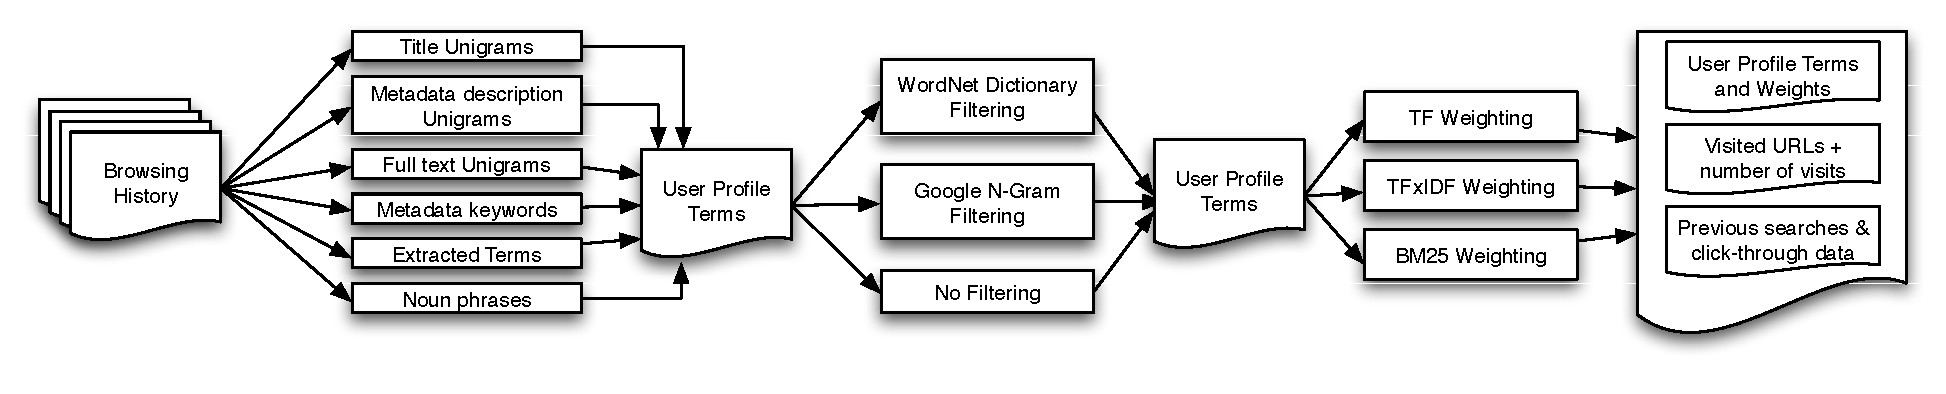
\epsfig{file=flowchart.eps, width=7in}
\caption{User Profile Generation Steps and Workflow}
\label{fig:workflow}
\end{figure*}

\subsubsection*{Click-through Based Approaches}

A different range of personalization strategies utilize URL and click-through data from past queries. In \cite{Joachims:Opt}, user click-through data is collected as training data to learn a retrieval function, which is used to produce a customized ranking of search results that suits a group of users' preferences. In \cite{Sugiyama:Hatano, Speretta:Gauch, Sun:Zeng}, the click-through data collected over a long time period is exploited through query expansion to improve retrieval accuracy. The most promising URL and click-through based method seems to be PClick, or person-level re-ranking based on historical clicks, as suggested in \cite{Dou:Song}. If a query is issued by a user for the second time, pages that have been clicked during the first search for this query are promoted to the top of the ranking. A disadvantage of this approach is that it can only be applied to repeated queries. The method suggested in this paper will incorporate both a user profile and a user's URL and click-through history. We compare our approach to the PClick method in section 5, and find obtain significant improvements.

\subsubsection*{Commercial Personalization Systems}

Recently, personalized search has also been made available in some of the mainstream web search engines including  Google\footnote{http://googleblog.blogspot.com/2009/12/personalized-search-for-everyone.html} and Yahoo!. These appear to use a combination of explicitly and implicitly collected information about a user. They allow the user to build a profile of themselves by selecting categories of interests and custom tailor the results delivered to the user based on that. However, in practice we expect few users to provide this explicit information. Implicitly, users' search and click-through history is also used personalize results, with results closer to that geographical location of the user additionally favored. However, as the details of these methods and algorithms are not publicly available, we only compare our approach to the default search engine ranking and not the personalized version.

\section{Personalization Strategies}

In this section, we describe our personalization approach. The first step consists of constructing a user profile, that is then used in a second phase to re-rank search results.

\subsection{User Profile Generation}

A user is represented by a list of terms and weights associated to those terms, a list of visited URLs and the number of visits to each, and a list of past search queries and pages clicked for these search queries. This profile is generated as shown in Figure \ref{fig:workflow}. First, a user's browsing history is collected and stored as (URL, HTML content) pairs. Next, this browsing history is processed into six different summaries consisting of term lists. Next, the terms can be filtered, and finally term weights are generated using three different weighting algorithms. We now describe each of these steps in detail.

\subsubsection{Data Capture}

%\begin{table}
%\centering
%\caption{Participant Statistics}
%\begin{tabular}{|l|c|} \hline
%\textbf{Metric}&\textbf{Total}\\ \hline
%Participants&50\\ \hline
%Data Capturing Period (Days)&92\\
%\hline\end{tabular}
%\end{table}

To obtain user browsing histories, a Firefox add-on called AlterEgo\footnote{The source code for this add-on can be downloaded from  http://github.com/nicolaasmatthijs/AlterEgo} was developed. To respect a user's privacy as much as possible, a random unique identifier is generated at installation time. This identifier is used for all data exchange between the add-on and the server recording the data\footnote{Note that it is necessary for this data to be collected by our server for research purposes, but our approach does not require this data to be centralized. Our entire method can execute client-side, avoiding the privacy concerns that otherwise arise with server-based approaches.}. Participants for this study were recruited via a website explaining the purpose and consequences to potential users, publicized on various e-mail lists, resulting in 50 participants taking part. Whilst we expect that most of these participants are employed in the IT industry due to the recruitment process, a number of people outside of the IT industry without significant web search experience participated as well.

Every time a user with this add-on installed leaves a non-secure (non-https) web page, the add-on transmits the current user's unique identifier, the URL of the page, the time that was spent on the page, the current date and time, and the length of the source HTML to the server. The server then adds the record to a queue of items to process. The server attempts to fetch the source HTML of all pages in the queue. This is performed server-side to ensure that only publicly-visible data is used. Once the source HTML is received, the server compares its length to the length received from AlterEgo. If the length difference is smaller than 50 characters, the HTML is accepted and saved along with the unique identifier, URL, duration and date and time into the database. Otherwise,  we assume the content probably came from a password protected but non-secure site (e.g. FaceBook, Hotmail etc.) and the record is discarded.

\begin{table}
\centering
\caption{Captured Data Statistics}
\begin{tabular}{|l|c|c|c|c|} \hline
\textbf{Metric}&\textbf{Total}&\textbf{Min}&\textbf{Max}&\textbf{Mean}\\ \hline
Page Visits&530,334&51&53,459&10,607\\ \hline
Unique Page Visits&218,228&36&26,756&4,364.56\\ \hline
Google Searches&39,838&0&4,203&797\\ \hline
Bing Searches&186&0&53&3.72\\ \hline
Yahoo Searches&87&0&29&1.74\\ \hline
Wikipedia Pages&1,728&0&235&34.56\\
\hline\end{tabular}
\label{tab:stats}
\end{table}

The add-on captured data for three months from March to May 2010. As shown in Table \ref{tab:stats}, a total of 530,334 page visits (or an average of 10,607 page visits per user) were recorded. 58\% of the visits were to unique pages. The add-on also recorded 39,838 Google searches, 186 Bing searches and 87 Yahoo! searches, indicating that our users are strongly biased towards Google as their search engine, hence Google is used as the baseline in our experiments. An average user issued 797 queries over the three months, indicating that at least 7.5\% of all web requests are search related.

\subsubsection{Data Extraction}

We considered the following summaries of the content viewed by users in building the user profile:
\vspace{3mm}

\noindent{\bf Full Text Unigrams}

The body text of each web page, stripped of html tags.

\vspace{1mm}
\noindent{\bf Title Unigrams}

The words inside any \emph{<title>} tag on the html pages.

\vspace{1mm}
\noindent{\bf Metadata Description Unigrams}

The content inside any \emph{<meta name="description">} tag on the html pages.

\vspace{1mm}
\noindent{\bf Metadata Keywords Unigrams}

The content inside any \emph{<meta name="keywords">} tag on the html pages.

\vspace{1mm}
\noindent{\bf Extracted Terms}

\begin{table}
\centering
\caption{Extracted terms from the AlterEgo website and the Wikipedia page about Mallorca}
\begin{tabular}{|c||c|} \hline
\textbf{AlterEgo}&\textbf{Mallorca}\\ \hline
add-ons&majorca\\ \hline
addons&island\\ \hline
Nicolaas&palma\\ \hline
Matthijs&islands\\ \hline
CSTIT&spanish\\ \hline
Nicolaas Matthijs&balearic\\ \hline
Cambridge&mallorca\\ \hline
Language Processing&cathedral\\ \hline
Google&Palma de Mallorca\\ \hline
keyword extraction&port\\
\hline\end{tabular}
\end{table}

We implemented the Term Extraction algorithm based on Unithood And Termhood Unification as presented in \cite{Vu:Ti}, running it on the full text of each visited web page. This algorithm uses the C/NC method, which uses a combination of linguistic and statistical information to score each term. Term candidates are found using a number of linguistic patterns and are assigned a weight based on the frequency of the term and its subterms. This is supplemented with term re-extraction using the Viterbi algorithm. The outcome of this algorithm run on two sample web pages can be seen in Table 3.

\vspace{1mm}
\noindent{\bf Noun Phrases}

Noun phrases were extracted by taking the text from each web page and splitting it into sentences using a sentence splitter from the OpenNLP Tools\footnote{http://opennlp.sourceforge.net/}. The OpenNLP tokenization script was then run on each sentences. The tokenized sentences were then tagged using the Clark \& Curran Statistical Language Parser\footnote{http://svn.ask.it.usyd.edu.au/trac/candc/wiki} \cite{Clark:Curran}, which assigns a constituent tree to the sentence, part of speech tags to each word. Noun phrases were then extracted from this constituent tree.

%Other ways to identify noun-phrases include using a dictionary on the source text and filter out all of the words that are not recognized as a noun. However, this might suffer from proper nouns not being in the dictionary. Another possible issue are words which can be used as multiple parts of speech being allowed in even though they're not used as a noun in the current context. It also does not succeed in extracting noun phrases from the text, which might be useful. For example ``web development" is more accurate in describing a person's interests than "web" and "development".

\subsubsection{Term List Filtering}

To reduce the number of noisy terms in our user representation, we also tried filtering terms using two different approaches. 

The first is dictionary filtering using the lexical database WordNet 3.0\footnote{http://wordnet.princeton.edu/}, retaining only words marked as nouns. However, WordNet is far from complete and hence tends to remove many nouns words, in particular most proper nouns.

The alternative way we tried was removing uncommon words using the Google N-Gram corpus\footnote{http://googleresearch.blogspot.com/2006/08/all-our-n-gram-are-belong-to-you.html}. This approach is general successfully remove non-sensical word, while allowing less common nouns such as proper nouns. However, as part of speech tags are not a part of the Google N-Gram corpus, it could not filter out stop words and determiners.

\subsubsection{Term Weighting}

After the list of terms has been accumulated and potentially filtered, we computed weights for each term using three methods.

\vspace{3mm}
\noindent{\bf TF Weighting}

The most straightforward implementation we consider is Term Frequency (TF) weighting. We define a frequency vector \begin{math} \vec{F} \end{math} that contains the frequency counts of a given term \begin{math} t{_{i}} \end{math} for all of the input data sources, as shown in equation (1). For example, \begin{math} f{_{title}} \end{math} is the number of times a given term \begin{math} t{_{i}} \end{math} occurs in all of the titles in the user's browsing history.  We calculate a term weight based on the dot product of these frequencies with a weight vector $\vec{\alpha}$:
\begin{eqnarray}
\vec{F}{_{t_i}} = \left[ \begin{array}{ccc}
f{_{title{_{t_i}}}} \\
f{_{mdesc{_{t_i}}}} \\
f{_{text{_{t_i}}}} \\
f{_{mkeyw{_{t_i}}}} \\
f{_{terms{_{t_i}}}} \\
f{_{nphrases{_{t_i}}}} \\
\end{array} \right]
\end{eqnarray}

\begin{eqnarray}
w{_{TF}}(t{_{i}}) & = & \vec{F}{_{t{_{i}}}} \cdot \vec{\alpha}
\end{eqnarray}

For simplicity, in our experiments we limit ourselves to three possible values for each weight $\alpha_i$: 0, ignoring the particular data field, 1, including the particular data field, and $\frac{1}{N_i}$, where $N_i$ is the total number of terms in field $i$. This gives more weight to terms in shorter fields (such as the meta keywords or title fields). We call the latter \emph{relative weighting}.

\vspace{3mm}
\noindent{\bf TF-IDF Weighting}

The second possibility for term weights we consider is TF-IDF (or Term Frequency, Inverse Document Frequency) weighting. Here, words appearing in many documents are down-weighted by the inverse document frequency of the term:
\begin{eqnarray}
w{_{TFIDF}}(t{_{i}}) & = & \frac{1}{log(DF{_{t{_{i}}}})} \times w{_{TF}}(t{_{i}})
\end{eqnarray}

To obtain IDF estimates for each term, we use the inverse document frequency of the term on all web pages using the Google N-Gram corpus.

\vspace{3mm}
\noindent{\bf Personalized BM25 Weighting}

The final weight method we consider is taken from Teevan et al \cite{Teevan:Main}. They propose a personal term weight similar to how BM25 weights terms. Specifically, they propose a weight
\begin{eqnarray}
w{_{BM25}(t{_{i}}}) & = & log\frac{(r{_{t{_{i}}}}+0.5)(N-n{_{t{_{i}}}}+0.5)}{(n{_{t{_{i}}}} + 0.5)(R-r{_{t{_{i}}}}+0.5)}, 
\end{eqnarray}

where \emph{N} represents the number of documents on the web (estimated from the Google N-Gram corpus, 220,680,773), $n{_{t_i}}$ is the number of documents in the corpus that contain the term $t_i$ (estimated using the Google N-Gram corpus), \emph{R} is the number of documents in the user's browsing history and $r_{t_i}$ is the number of documents in the browsing history that contains this term within the selected input data source. 

While this method allows us to compare our results against the approach proposed by Teevan et al., note that we do not have access to users' full Desktop index, and are limited to their browsing history, making our implementation potentially less effective.

\subsection{Re-ranking Strategies}

Like previous work, we use the user profile to re-rank the top results returned by a search engine to bring up results that are more relevant to the user. This allows us to take advantage of the data search engines use to obtain their initial ranking to first obtain a small set of results that can then be personalized. In particular, \cite{Teevan:Main} noted that chances are high that even for an ambiguous query the search engine will be quite successful in returning pages for the different meanings of the query. We opt to retrieve and re-rank the first 50 results retrieved for a query. Each of these 50 search results is given a weight and are re-ranked accordingly. 

\subsubsection{Weighting Methods}

When reranking, each candidate document can either be scored, or just the snippets can be scored. We focus on assigning scores to the search snippets as it was found to be more effective for re-ranking search results by Teevan et al.~\cite{Teevan:Main}. Also, using search snippets allows a straightforward client-side implementation of search personalization. We implemented the following four different weighting methods:

\vspace{3mm}
\noindent{\bf Matching}

For each word in the search snippet's title and summary that is also in the user's list of profile terms, the weight associated with that term will be added to the snippet's weight: 
\begin{eqnarray}
score_{M}(s_i) & = & \sum_{z = 0}^{N_{s_i}} f{_{t_i}} \times w(t_z)
\end{eqnarray}

where $N_{s_i}$ represents the total number of unique words within the snippet's title and summary, and $f_{t_i}$ represents the number of occurrences of $t_i$ within the snippet. Words in the snippet title or summary but not in the user's profile do not contribute towards the final weight. This method is equivalent to taking the dot product between the user profile vector and the snippet vector.

\vspace{3mm}
\noindent{\bf Unique Matching}

A second search snippet weighting option we consider involves counting each unique word just once:
\begin{eqnarray}
score{_{UM}}(s_i) & = & \sum_{z = 0}^{N_{s_i}} w(t_z)
\end{eqnarray}

\vspace{3mm}
\noindent{\bf Language Model}

The third weight calculation method attempts to generate a unigram language model from the user profile in which the weights associated to the terms are used as the frequency counts for the language model:
\begin{eqnarray}
score{_{LM}}(s{_{i}}) & = & log( \prod_{z = 0}^{N{_{s{_{i}}}}} \frac{w(t{_{z}}) + 1}{w{_{total}}}) \nonumber \\
& = & \sum_{z = 0}^{N{_{s{_{i}}}}} log(\frac{w(t{_{z}}) + 1}{w{_{total}}})
\end{eqnarray}

where \emph{N} is the total number of words in the snippet's title and summary, and \begin{math} w{_{total}} \end{math} stands for the sum of all the weights within the user profile. The language model estimates the probability of a snippet given a user's profile. To avoid a zero probability for snippets that contain words not in the user's profile, we use add-1 smoothing.

\vspace{3mm}
\noindent{\bf PClick}

As a final snippet weighting method we use the PClick algorithm proposed by Dou et al.~\cite{Dou:Song}. It assumes that for a query \emph{q} submitted by a user \emph{u}, the web pages frequently clicked by \emph{u} in the past are more relevant to \emph{u}. The personalized score for a snippet is: 
\begin{eqnarray}
score_{PC}(s{_{i}}) & = & \frac{|Clicks(q,p,u)|}{|Clicks(q,\bullet ,u)| + \beta}
\end{eqnarray}

where \begin{math} |Clicks(q,p,u)| \end{math} is the number of clicks on web page \emph{p} by user \emph{u} for query \emph{q} in the past, \begin{math} |Clicks(q,\bullet ,u)| \end{math} is the total click number on query \emph{q} by  \emph{u}, and \begin{math} \beta \end{math} is a smoothing factor set to 0.5.
Note that PClick makes no use of the terms and weights associated to the user's profile and is solely based on click-through data for a given query. As such, it only affects repeated queries.

\subsubsection{Additional Options}

Finally, we consider two adjustments to the snippet scores. First, we consider giving additional weight to URLs that have been visited previously. This extends PClick in that it boosts \emph{all} URLs that have previously been visited, while PClick only boosts URLs that have directly been clicked for the current search query. The snippet weight will be boosted by the number of previous visits to that web page (\emph{n}) times a factor $v$:
\begin{equation}
\mathrm{finalScore}(s_i) = score(s_i) * (1 + v \times n_i)
\label{eqn:visited}
\end{equation}

Second, in the re-ranking framework discussed so far, the original ranking is not taken into account. The original rank can be incorporated into the final snippet weight by multiplying the snippet weight by the inverse log of the snippet's original rank $r_{s_i}$:
\begin{equation}
\mathrm{finalScore}(s_i) = score(s_i) \times \frac{1}{log(r_{s_i})}
\end{equation}

We expect both these extensions to be very beneficial.

\section{Evaluation Approach}

We now consider potential evaluations for personalized search strategies. On the one hand, offline approaches allow the creation of a standard dataset that can be used to optimize personalization parameters. On the other hand, only an online test with actual users can truly reflect how changes to rankings affect user behavior. We now explore the available alternatives, and describe our final strategy.

\subsubsection*{Relevance judgements}

The first offline evaluation approach (e.g.~used by Teevan et al.~\cite{Teevan:Main}) is based on assembling a group of people that judge the relevance of the top \emph{k} documents or search snippets for a set of queries. Given these relevance judgements, a standard metric such as  (N)DCG or (Normalized) Discounted Cumulative Gain \cite{ADD} can be calculated for a given query and ranking, reflecting the quality of the presented ranking for that user. This approach has the advantage that once the relevance judgements are made, it allows for testing many different user profile and re-ranking parameter configurations. However, due to the long time it takes to judge \emph{k} documents, this can only be done for a small number of search queries. As volunteers need to be found to sit through this slow and tedious evaluation process, it is also hard to gather a large group of evaluators. The evaluation process also does not reflect a user's normal browsing and searching behavior, which might influence the final results. Moreover, this approach assumes that (N)DCG is the right way to combine a set of relevance judgements into a rank quality score. Finally, the queries evaluated must be representative of a true query load, or offline results may not reflect perhaps poorer performance for non-personalizable queries. 

\subsubsection*{Side-by-side evaluation}

An alternative offline evaluation method, previously used for example by \cite{Thomas:Hawking}, consists of presenting users with two alternative rankings side-by-side and ask which they consider best. The advantage of this method is that an actual judgement is made of which ranking is the best one, although users evaluate the entire presented ranking whilst in real life situations they might only look at the first couple of results, potentially biasing the results. Judging two rankings next to each other is considerably faster than judging \emph{k} documents per query, but it still requires a long offline evaluation exercise. Additionally, an evaluator has to provide a new assessment for each distinct ordering of documents that is investigated. This makes it hard to use such judgments to tune reranking parameters.

\subsubsection*{Clickthrough-based evaluation}

One online evaluation approach involves looking at the query logs and click-through data from a search engine on large scale (e.g.~used by \cite{Dou:Song}). The logs record which search result was clicked for a given query, allowing the evaluator to check if the clicked result would be positioned higher in a personalized ranking. This allows for testing many parameter configurations and also does not require any user effort as their actions are recorded as they go, reflecting their natural environment and browsing behavior. However, the method can have difficulties in assessing whether a search personalization strategy actually works. First, users are more likely to click a search result presented at a high rank, although these are not necessarily most or more relevant \cite{Joachims:Granka}. It is also unsuccessful in assessing whether the results that have been brought up from a page lower down would have been relevant as they would rarely have been clicked if originally shown at low rank. On top of that, we also have no access to such large scale usage and user profile data for this experiment.

Alternatively, both personalized and non-personalized rankings can be shown online to users, with metrics such as mean clickthrough rates and positions being computed. However, \cite{Radlinski:Kurup} showed that such an approach is not sensitive enough to detect small differences in relevance with thousands of query impressions as we could obtain in an online experiment.

\subsubsection*{Interleaved evaluation}

The final online evaluation option we consider, which to our knowledge has not been used before for the evaluation of personalized search, is interleaved evaluation \cite{Joachims:Thorsten, Radlinski:Kurup}. Interleaved evaluation combines the results of two search rankings by alternating between results from the two rankings while omitting duplicates, and the user is presented with this interleaved ranking. The ranking that contributed the most clicks over many queries and users is considered better. Radlinski et al.~\cite{Radlinski:Kurup} showed that this approach is much more sensitive to changes in ranking quality than other click-based metrics. It has also shown to correlate highly with offline evaluations with large numbers of queries \cite{Radlinski:Craswell}. On top of that, this method does not require any additional effort from the user, providing an evaluation users naturally use search engines. However, one evaluation only provides an assessment for one particular ranking, and thus an evaluation is required for each parameter configuration being investigated. It is also the hardest evaluation technique for showing improvements as, opposed to other metrics, bringing a slightly relevant page up from rank 8 to rank 5 will not help if the most relevant page is at rank 1.

\subsection{Evaluation Plan}

This last approach, interleaved evaluation, best reflects real user experience, and would be preferred for evaluating a personalized search system. However, the user profile generation and re-ranking steps both have a large number of possible parameters and it is infeasible to perform an online evaluation for all of them. Hence, we start with an offline NDCG based evaluation to pick the optimal parameter configurations that we then evaluate with the more realistic online interleaved evaluation.

\section{Offline Evaluation}

This section first describes how we collected relevance judgments for offline evaluation. Next, we describe how this was used to identify the most promising personalization strategies.

\subsection{Relevance Judgements}

To obtain personalized relevance judgments, six participants who had installed the AlterEgo plugin recording their browsing behavior were recruited. At that point, two months of browsing history had been recorded and stored for each of them. 

The process and format of the evaluation sessions was kept very similar to the relevance judgment session conducted by Teevan et al \cite{Teevan:Main}. Each participant was asked to judge the relevance of the top 50 web pages returned by Google for 12 queries according to the criteria presented in Table \ref{tab:guidelines}. The documents were presented in a random order. Full web pages were evaluated instead of snippets because the user is only interested in the actual web page being relevant for his information need.

Every participant was asked to provide 600 judgments, 50 relevance judgements for each of 12 queries. The first query participants were asked to judge was their own name (Firstname Lastname) as a warm-up exercise. Next, each participant was presented with a list of 25 general search queries in a random order, consisting of 16 queries taken from the TREC 2009 Web Search track queries and 9 other UK focussed queries such as ``pub", ``football" and ``cambridge". All users were asked to judge 6 of these queries. Examples of some of the queries chosen by multiple people can be seen in Table \ref{tab:queries}. Finally, each participant was presented with their most recent 40 search queries (from their browsing history) and were asked to judge 5 for which they remembered the returned results could have been better.

On average, it took each participant about 2.5 hours to complete this exercise. Particularly interestingly, all users mentioned that during to the exercise they came across really interesting websites which they did not know existed before, indicating that there is a potential for search personalization to enrich the set of returned results.

\begin{table}
\centering
\caption{Relevance judgements guidelines}
\begin{tabular}{|l|} \hline
(a) Select \emph{Irrelevant} if the document is not useful and\\
not interesting to you.\\
(b) Select \emph{Relevant} if the document is interesting to you,\\
but is not directly about what you were hoping to find\\
or if the document is somewhat useful to you, meaning\\
that it touches on what you were hoping to find\\
(maximum 1 paragraph), but not very extensively.\\
(c) Select \emph{Very Relevant} if the document is useful or very\\
interesting to you, i.e. it is what you were hoping to find.\\
\hline\end{tabular}
\label{tab:guidelines}
\end{table}

\begin{table}
\centering
\caption{Common queries used by different participants}
\begin{tabular}{|l|c|} \hline
\textbf{Query}&\textbf{Users}\\ \hline
Cambridge&6\\ \hline
GPS&4\\ \hline
Website design hosting&3\\ \hline
Volvo&3\\
\hline\end{tabular}
\label{tab:queries}
\end{table}

\subsection{Results and Discussion}

The following parameters were investigated for profile generation, representing the different steps shown in Figure 1:

\begin{itemize}
\item All combinations of the six different input data sources with three possible values for $\alpha$ (namely 0, 1 and normalized)
\item Three filtering methods: No Filtering, WordNet noun filtering and Google N-Gram filtering using a threshold of 1,000
\item The three term weighting methods: TF, TF-IDF and BM25
\end{itemize}

In terms of re-ranking the search results, the following set of parameters were investigated: 

\begin{itemize}
\item The four snippet weighting methods: Matching, Unique Matching, Language Model and PClick
\item Whether or not to consider the original Google rank
\item Whether or not to give extra weight to previously visited URLs (using $v=10$)
\end{itemize}

For every profile and ranker combination, the mean personalized NDCG was measured as follows:

\begin{equation}
NDCG@p = {1 \over Z} \sum_{i = 1}^{p} \frac{2^{rel_i} - 1}{\log_2(1 + i)}
\label{eqn:ndcg}
\end{equation}

where $rel_i$ is determined from the relevance judgements (non-relevant = 0, relevant = 1 and very relevant = 2) and $Z$ is such that the maximum NDCG for each query is 1. In all of these following results, we compare NDCG scores that have been averaged across all queries and all users.

\subsubsection{Baseline Comparisons}

\begin{figure}
\centering
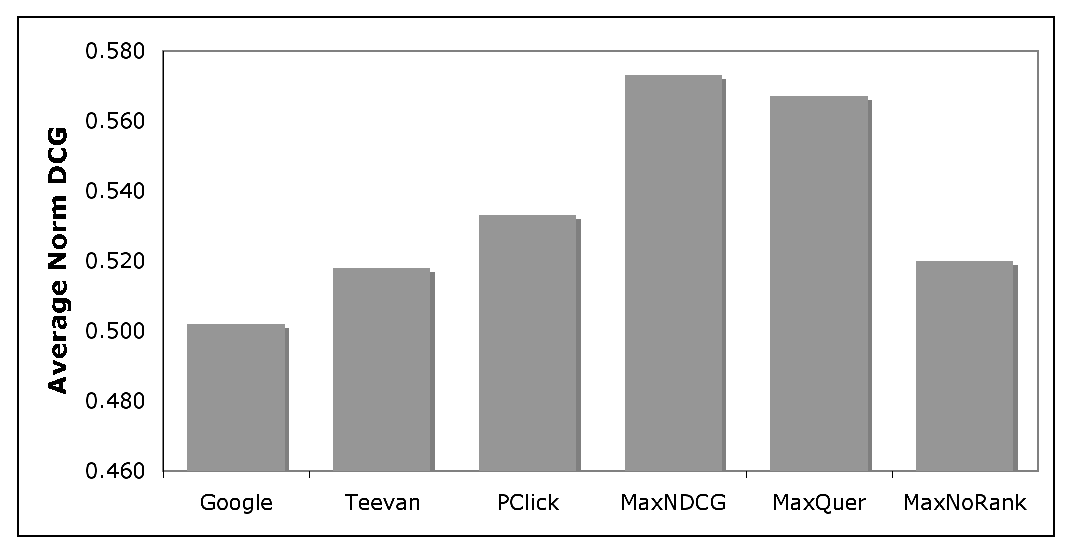
\epsfig{file=graph1.eps, width=3in}
\caption{Average Normalized DCG scores comparing baseline system performance to best personalization strategies}
\label{fig:ndcg}

\centering
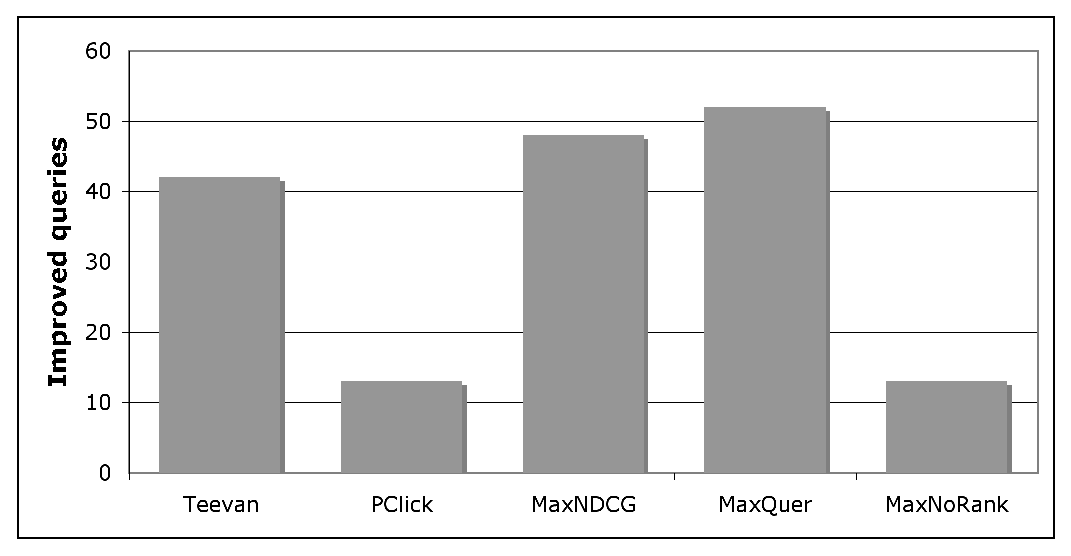
\epsfig{file=graph2.eps, width=3in}
\caption{Comparing baseline system performance to best personalization strategies in terms of number of improved queries}
\label{fig:queries}
\end{figure}

To assess how well our different personalization strategies performed, we compared the outcome of the experiment with several baselines as shown in Figures \ref{fig:ndcg} and \ref{fig:queries}. The reported scores are normalized DCG scores for all 72 queries, and all statistical analyses were performed using a paired T-Test.

%\begin{table}
%\centering
%\caption{Number of strategies that improve over the default Google ranking}
%\begin{tabular}{|l|c|c|} \hline
%\textbf{Baseline}&\textbf{Better}&\textbf{Consistently Better}\\ \hline
%Google&4,455&1,556\\ \hline
%Teevan&3,335&413\\ \hline
%PClick&1,580&359\\
%\hline\end{tabular}
%\label{tab:counts}
%\end{table}

The baseline methods we compare to are the default Google ranking, the Teevan method and the PClick method. The results obtained appear to agree with those reported in \cite{Teevan:Main} and \cite{Dou:Song}. We find the Teevan approach is significantly (p < 0.05) better than Google and PClick is significantly (p < 0.01) better than Google. Note that in our implementation of the Teevan algorithm we only make use of the browsing history as input data, as we do not have access to the user's files or e-mails, which may disadvantage it.

%As shown in Table \ref{tab:counts}, out of the 15,878 user profile and re-ranking combinations that have been investigated, a total of 4,455 combinations performed better than Google. 1,556 combinations performed consistently better than Google, meaning that the average NDCG score for each user was higher than Google, indicating that the personalization strategy worked for all six users. A total of 3,335 strategies performed better than the Teevan approach, of which 413 were consistently better. Compared to PClick, 1,580 combinations performed better of which 359 were consistently better.

\newcommand{\MaxNDCG}{{\tt MaxNDCG}}
\newcommand{\MaxQuer}{{\tt MaxQuer}}
\newcommand{\MaxNoRank}{{\tt MaxNoRank}}
\newcommand{\MaxBestPar}{{\tt MaxBestPar}}

\begin{table*}
\centering
\caption{Investigated profiles for interleaved evaluation}
\begin{tabular}{|l|l|c|c|} \hline
\textbf{Name}&\textbf{Method}&\textbf{Avg NDCG}&\textbf{Improved}\\ \hline
{\MaxNDCG}&TF-IDF, RTitle, RMKeyw, RCCParse, NoFilt - LM, Look At Rank, Visited&0.573&48/72\\ \hline
{\MaxQuer}&TF, RTerms, RCCParse, NoFilt - LM, Look At Rank, Visited&0.567&52/72\\ \hline
{\MaxNoRank}&TF, RMKeyw, NoFilt - LM, Look At Rank, Visited&0.520&13/72\\ \hline
{\MaxBestPar}&BM25, RTitle, RMKeyw, RTerms, NoFilt - LM, Look At Rank, Visited&0.566&45/72\\
\hline\end{tabular}
\label{tab:selected}
\end{table*}

We selected four user profile and re-ranking parameter settings, summarized in Table \ref{tab:selects}, to further evaluate. The first, \MaxNDCG, yielded the highest average NDCG score on the offline dataset. It involves using Title, Metadata Keywords and Extracted noun phrases as input data using relative weighting, no filtering, and TF-IDF as the weighting method. The second, \MaxQuer had the highest number of improved queries. It consisted of using Extracted Terms and Extracted noun phrases as input data using relative weighting, no filtering and TF as the weighting method. The third, \MaxNoRank, was the best method that does not take the original Google ranking into account. It uses Metadata keywords as input data, no filtering and TF as the weighting method. Finally, \MaxBestPar was obtained by a greedy selection strategy in each parameter was selected one at a time and then locked. It is very similar to \MaxNDCG, consisting of using Title, Metadata Keywords and Extracted Terms as input data using relative weighting, no filtering and BM25 for term weight calculation. All of these selected profiles used Language Model snippet weighting, the Google rank was taken into account and previously visited URLs received addition weight per Equation \ref{eqn:visited} with $v=10$.

\MaxNDCG and \MaxQuer are both significantly (p < 0.01) better than default Google, Teevan and PClick. \MaxNDCG, with an average NDCG of 0.573, yields a 14.1\% improvement over Google, and \MaxQuer, with an average NDCG of 0.567, yields a 12.9\% improvement over Google.

Interestingly, despite \MaxNoRank ignoring the Google rank, it obtaining an NDCG score of 0.520 that is significantly (p < 0.05) better than Google and better than Teevan. A ranking that outperforms web ranking based on user data has to our knowledge not yet been achieved. While this may be a result of overfitting the parameters given our small offline dataset, we observed this effect often that we do not believe this to be the case.

A different metric that can be used for comparison of personalization methods is to look at the number of queries for which the NDCG score improved, as shown in Figure \ref{fig:queries}. PClick improves fewest, 13 out of 72 queries, compared to the 44 improved queries for the Teevan approach, despite obtaining a higher NDCG score. This is because the PClick method only works on repeated queries by bringing up pages on which the user previously clicked. While this will only occasionally cause personalization, it makes bigger improvements when it reranks results. Also, the Teevan approach has a negative effect on some of the queries as well. \MaxNDCG improves performance on 48 queries, \MaxQuer improves 52. 

\subsubsection{Parameter Configuration}

\begin{figure*}
\centering
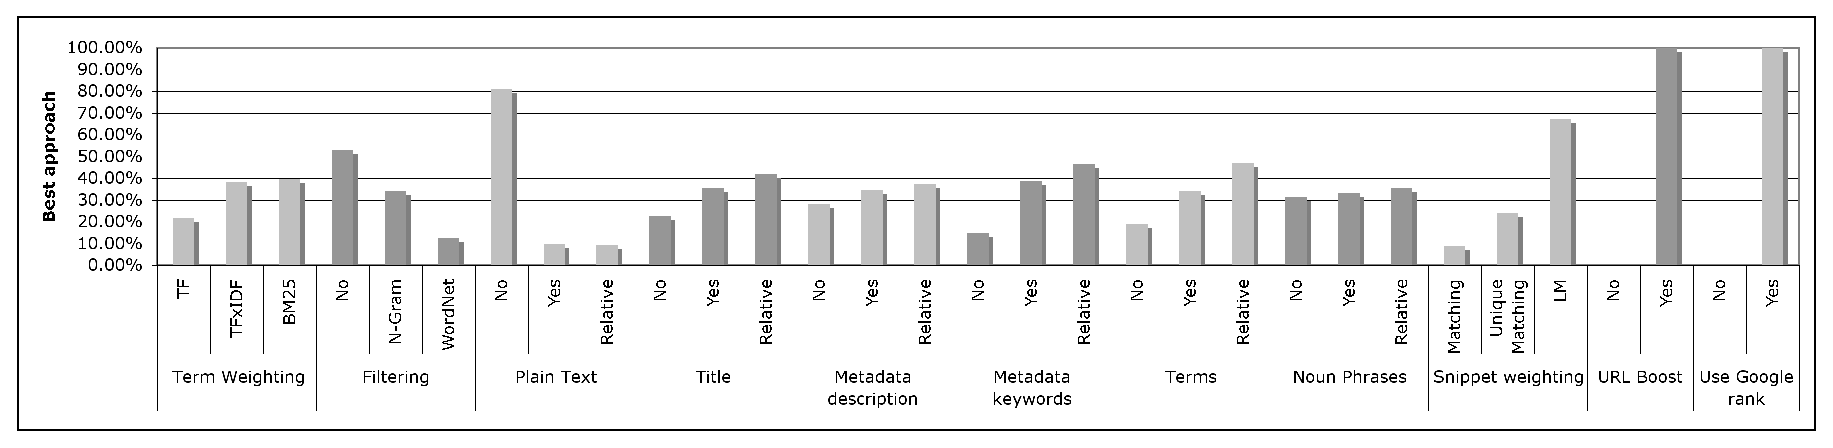
\epsfig{file=graph6.eps, width=6in}
\caption{Percentage-wise number of times an investigated parameter performs best for a given parameter configuration}
\label{fig:perparam}
\end{figure*}

Given all the investigated user profile and re-ranking combinations, we look at how all of these parameters alter the overall strategy performance. We summarize the one-way effects of all individual parameters and explore their influence on the average NDCG score. In Figure \label{fig:perparam}, we consider a certain parameter $\lambda$ (e.g. filtering, term weighting, etc.). For every other parameter setting, we counted how often the different possible values of $\lambda$  were most helpful. We repeated this experiment for every parameter group. These approaches do not examine interaction effects, so at the end of this section we give an overview of which parameter combinations achieved the best performance. Note that most parameters only make a small difference in NDCG, even if they are preferred in most cases.

In terms of re-ranking strategies, it is clear that there is one approach that significantly outperforms all other ones, indicating that this approach should be used for all generated profiles. Using the Matching approach for snippet weight calculation is significantly worse (p < 0.01) than using Unique Matching. Using a Language Model based on the user profile performs significantly better (p < 0.01) than both Matching and Unique Matching and is in 67\% of the investigated profiles the best choice. Unique Matching only occasionally performs better than a Language Model when the user profile is very much keyword based and does not use Extracted Nouns, Title, etc. as input data. Except for a single case, multiplying the snippet weight by 10 for URLs that have previously been visited performs significantly better (p < 0.01) than not keeping this into account. This proves that a combination of a user profile based and click based personalization strategy can be used successfully. Not normalizing the obtained snippet weights by their original rank always performs worse than when the Google rank is taken into account.

When looking at the input data used to generate a user's profile, it can be seen that all data sources are helpful in improving personalization performance, except when the full web page text is used. Not using the full text performs significantly better (p < 0.01) than when this is included. This indicates that treating web pages like a normal document or a bag of words does not work, presumably due to its noisy nature. Using metadata keywords, extracted terms and the page title all yield significant (p < 0.01) improvements over not including them. Metadata description and extracted noun phrases also give a significant (p < 0.05), but less strong, improvement. The different input data sources can be ranked in terms of helpfulness for personalization: metadata keywords, extracted terms, title, metadata description and extracted noun phrases. However, a combination of the most helpful data sources does not necessarily achieve the best performance, as strong parameter interactions exists between the different sources. It can also be seen that using relative weighting performs consistently better than giving every term of every data source a weight of 1. This can be explained by the fact that the most helpful data sources are the ones that contain the lowest number of terms, becoming more numerous as the data sources become less helpful.

The charts show that in general no term filtering performs significantly better (p < 0.01) than using Google N-Gram based filtering, which in its turns performs significantly better (p < 0.01) than WordNet noun filtering. WordNet filtering seems to filter out too many actual relevant terms, which is reflected in its lower average NDCG score. Even though no filtering performs significantly better than Google N-Gram filtering, the actual difference in NDCG score is very small (0.001), which can be explained by the fact that N-Gram filtering only filters out non-sensical terms, which are rare in snippets, and not the words that harm in personalization.

When looking at term weighting methods, it seems that Term Frequency performs significantly worse (p < 0.01) than TF-IDF and BM25. BM25 performs on average significantly better (p < 0.05) than TF-IDF. However, when looking at the number of times a given parameter value is the best option for a parameter configuration, we can see that TF-IDF and BM25 are the best option for roughly the same number of approaches. BM25 seems to work better in general when the input data is richer and thus noisier, as it normalizes the term weights. TF-IDF is in general more successful when the selected set of input sources are more keyword focussed.

\subsubsection{Relevance Distribution}

\begin{figure*}
\centering
\epsfig{file=graph3a.eps, width=7in}
\caption{Distribution of relevance at rank for the Google and {\tt MaxNDCG} rankings}
\label{fig:relDist}
\end{figure*}

Of the 3,600 relevance judgements collected in the evaluation session, 9\% were Very Relevant, 32\% Relevant and 58\% as Non-Relevant. The relevance judgements distribution for the default Google rank and the {\tt MaxNDCG} re-ranking approach shown in Figure \ref{fig:relDist} indicates that web rank already manages to place the biggest part of the Very Relevant results in the top 5 results. However, the relevance distribution for the {\tt MaxNDCG} strategy shows that personalized search manages to add more Very Relevant results into the top 5 of the ranking, but it mainly succeeds in adding Very Relevant results in between rank 5 and 10. This is expected as the personalization strategy keeps the Google rank into account and is thus less aggressive at very high ranks.

The Relevant results are evenly spread over all ranks, with slightly more weight towards the first half of the ranking. The personalization strategy manages to add a few more Relevant results to the top 5 of the different rankings. Irrelevant results are present at all ranks, but become more dominant after rank 10. Personalized search manages however to remove quite a large number of Irrelevant results out of the top 10 results and pushes them down into the lower regions of the rankings.

\subsubsection{Selected Profiles}

Given the discussed results, we selected 3 promising profiles to carry on with in the interleaved evaluation experiment. The chosen profiles are {\tt MaxNDCG}, as it yielded the highest normalized NDCG, {\tt MaxQuer}, as it improved on most queries and {\tt MaxBestPar} as it uses the best parameters according to our greedy learning approach. All of these selected profiles use Language Model snippet weighting, take into account the Google rank, and multiply the weight of previously visited URLs by 10 and the number of visits.

\section{Online Evaluation}

The second stage in the evaluation process is a large scale online interleaved evaluation. It is very important that this evaluation is run over a long enough period of time to get a sufficient number of queries per user, and that a reasonable amount of users participate in order to get quantitative and reliable results. It is crucial that participants are able to do the evaluation during their day-to-day lives as realistic information needs come up. This attempts to assess whether any of the 3 personalization strategies selected in section 5 yield an actual improvement in a user's search experience. It is also critical that in doing this evaluation exercise, users' search experience is not altered and they no noticeable differences can be detected in the user interface.

In this section, we first describe the details of the large scale online interleaved evaluation. Next, we discuss the results obtained and find out what the best personalization strategy is and whether it improves over Google. ADD: Given our limited offline relevance data, if we didn't do this, we might overfit.

\subsection{Interleaving Implementation}

\renewcommand{\algorithmiccomment}[1]{\dotfill {\it \small #1}}
\begin{algorithm}[t]
\begin{algorithmic}[1]
\STATE {\bf Input}: Rankings $A = ( a_1, a_2, \dots)$ and $B = ( b_1, b_2,
\dots)$
\STATE {\bf Init}: $I \leftarrow (); TeamA \leftarrow \emptyset; TeamB
\leftarrow \emptyset;$
\WHILE {($\exists i: A[i] \not\in I) \wedge (\exists j: B[j] \not\in I)$}
  \IF{$(|TeamA| < |TeamB|) \vee\newline \hspace*{0.35cm} ((|TeamA| \!=\!
|TeamB|) \wedge (RandBit()\!=\!1))$}
    \STATE $k \leftarrow \min_i\{ i : A[i] \not\in I \}$\COMMENT{top result in
A not yet in I}
    \STATE $I \leftarrow I+A[k];$\COMMENT{append it to I}
    \STATE $TeamA \leftarrow TeamA \cup \{A[k]\}$\COMMENT{clicks credited to A}
  \ELSE
    \STATE $k \leftarrow \min_i\{ i : B[i] \not\in I \}$\COMMENT{top result in
B not yet in I}
    \STATE $I \leftarrow I+B[k]$\COMMENT{append it to I}
    \STATE $TeamB \leftarrow TeamB \cup \{B[k]\}$\COMMENT{clicks credited to B}
  \ENDIF
\ENDWHILE
\STATE {\bf Output}: Interleaved ranking $I$, $TeamA$, $TeamB$
\end{algorithmic}
\caption{Team-Draft Interleaving} \label{alg:teamdraft}
\end{algorithm}

Therefore, an updated version of the AlterEgo Firefox add-on was developed and all of the volunteers who downloaded and installed the initial version were asked to upgrade to this second version. The add-on detects when a user submits a web search via Google and sends the search query, the unique user identifier and the current page number over to the server. Next, the server requests the first 50 search results from Google for the given query and picks one of the three personalization strategies at random. The selected strategy is used to calculate the snippets weights and re-ranking is done accordingly.

In our experiments, we use the Team-Draft interleaving algorithm, as described in Algorithm \ref{alg:teamdraft}, to interleave the original Google ranking and the re-ranked personalized version. This algorithm is motivated by how sports teams are often assigned in friendly games. Given a pool of available players (ranking A and B), two captains (one for TeamA and one for TeamB) take turns picking their next favorite player in the set of remaining players, subject to a coin toss every turn deciding which team captain gets to pick first. More details about this approach can be found in \cite{Radlinski:Kurup}. The combined ranking is presented to the user and clicks on any of the results are recorded. If results from the personalized ranking end up being clicked more often, it is a strong indicator that the personalization is successful.

The Team-Draft interleaving algorithm, as described in Algorithm 1, is then utilized to interleave the original Google ranking with the new personalized re-ranked version. In doing this, 50\% of the search results are assigned to Team A, which represents the default Google ranking, and 50\% is assigned to Team B, which represents the personalized ranking. A click that is recorded for either of these teams is considered a vote for the ranking they represent. The interleaved results are sent back to the user's browser, where they replace the original list of results, but keeping the surrounding page elements and thus not altering the search environment.

To avoid presenting slightly different rankings every time a search page is refreshed, both the random personalization strategy selector and the random bit inside the interleaving algorithm were seeded with a combination of unique identifier, query and the current hour.

An additional user experience consideration that had to be taken into account was re-ranking performance. A user profile had an average size of about 3.4 Megabyte, and all of them were kept in memory for fast access. Also, the user profiles were automatically updated on an hourly basis.

\subsection{Results and Discussion}

\begin{table}
\centering
\caption{Search Queries and Team votes per personalization strategy}
\begin{tabular}{|l|c|c|c|} \hline
\textbf{Method}&\textbf{Queries}&\textbf{Google Vote}&\textbf{Re-ranked Vote}\\ \hline
\MaxNDCG&590&220 (37.3\%)&370 (62.7\%)\\ \hline
\MaxQuer&621&295 (47.5\%)&326 (52.5\%)\\ \hline
\MaxBestPar&636&290 (45.7\%)&346 (54.3\%)\\
\hline\end{tabular}
\label{tab:votes}

\centering
\caption{Rank quality implications for each Personalization Strategy}
\begin{tabular}{|l|c|c|c|} \hline
\textbf{Method}&\textbf{Unchanged}&\textbf{Improved}&\textbf{Deteriorated}\\ \hline
\MaxNDCG&429 (67.5\%)&152 (23.9\%)&55 (8.7\%)\\ \hline
\MaxQuer&444 (71.6\%)&112 (18.1\%)&64 (10.3\%)\\ \hline
\MaxBestPar&403 (68.3\%)&128 (21.6\%)&59 (10.1\%)\\
\hline\end{tabular}
\label{tab:queryComp}
\end{table}

\begin{figure*}
\centering
\epsfig{file=graph7.eps, width=7in}
\caption{Rank differences for deteriorated (light grey) and improved queries (dark grey) for \MaxNDCG, \MaxQuer and \MaxBestPar}
\label{fig:rankChanges}
\end{figure*}

\begin{figure}
\centering
\epsfig{file=graph9.eps, width=3in}
\caption{Degree of personalization per rank}
\label{fig:byRank}
\end{figure}

In this section, we present the results from the interleaved evaluation experiment. We expect it to be harder to show actual improvements for this evaluation since bringing a relevant result up to a rank beneath the most relevant result will likely not make a difference in a user's behavior. This experiment should however give a clearer idea of whether our suggested personalization methods yield an improvement in real life. The previous evaluation phase also had a strong emphasis on ambiguous queries, whilst the share of ambiguous queries should be lower in this evaluation, making it harder to successfully deploy search personalization.

This interleaved evaluation experiment was run over three weeks, for the 41 users who updated the plugin. A total of 2,715 queries were submitted, of which 1,847 received an actual click on a search result. 76\% of these search queries were unique and 24\% were repeated queries.

Each click on a search result represented a vote for either the original Google ranking or the re-ranked personalized ranking and the user profile that was used to do the actual re-ranking. The total number of votes for each and each strategy can be seen in Table \ref{tab:votes}, showing that all of the investigated personalization approaches yield an actual improvement over the default Google ranking. \MaxNDCG significantly outperforms (p < 0.01) web ranking by more than both \MaxQuer and \MaxBestPar. \MaxQuer and \MaxBestPar both outperform web ranking as well, although their improvements are not statistically significant. The collected votes suggest that \MaxNDCG is the most convincing and best performing personalization strategy, which is in line with the findings from the first evaluation experiment. Although \MaxBestPar performs better than \MaxQuer in the current experiment, which is in contrast with the NDCG scores obtained in the relevance judgements session, the difference between these algorithms is not statitically significant.

The effect personalization has on the set of search queries for the different strategies can be seen in Table \ref{tab:queryComp}. The Unchanged column indicates the number of queries for which personalization did not make a difference, i.e. the clicked result was at the same rank for both the default ranking and the personalized ranking. The \emph{Improved} column shows the number of occasions in which the clicked result was brought up due to search personalization, whilst the \emph{Deteriorated} column shows the amount of queries for which the clicked result was lower in the ranking due to personalization. The trends that can be seen from the voting results are consistent with these numbers, however the actual differences between the different approaches seem smaller. On average, about 70\% of the search queries are untouched by search personalization, 20\% of the queries are improved and 10\% becomes worse. \MaxQuer seems like the least effective approach, having the highest percentage of unchanged queries, the highest percentage of deterioration and the lowest percentage of improvements. However, \MaxQuer still improves more queries than the ones it makes worse, indicating that it is still a successful approach. \MaxBestPar generally makes about the same number of queries worse, however its improvement percentage is 3.5\% higher than for \MaxQuer and it also leaves fewer search queries unchanged. \MaxNDCG again clearly seems to be the most successful personalization approach, having the highest change  and improvement rate and the lowest harming rate, improving 2.7 times more queries than it harms.

Figure \ref{fig:rankChanges} shows, for each of the personalization strategies, the distribution of rank changes for all queries that were improved or became worse. It can be seen that for large majority of the deteriorated queries, especially for {\tt MaxNDCG}, the clicked result only loses 1 rank compared to the original ranking. The majority of clicked results that improved a query gain 1 rank as well, however there are quite a few relevant results that are bumped up 2, 3, 4 or even 5 ranks. For each of the personalization strategies, the average rank deterioration is about 1.38 and the average rank improvement is around 3.5, indicating that the gains achieved by personalization are on average more than twice as high as the losses experienced on a query that was originally better. In other words, if personalization was unsuccessful for a query, a user could expect to find the result he was looking for at a rank which is on average only 1 lower than were it originally was. However, when personalization is successful, the result the user is looking for will on average be 3 or 4 ranks higher than original.

Figure \ref{fig:byRank} shows how much personalization is achieved through the suggested approaches at each rank. It can be seen that most re-ranking is done after rank 10, having little or no influence on user's search experience. Less actual re-ranking is done in the first 5 ranks due to the rank normalization going on, which has already proven to be a worthwhile approach. {\tt MaxQuer} does the least re-ranking in general, whilst {\tt MaxBestPar} does most re-ranking after rank 10.

In summary, it can be seen that the personalization strategy that uses Title, Metadata keywords and Extracted noun phrases as input data using relative weighting, no filtering and TF-IDF as the term weighting scheme, is the most effective according to both the voting method and the number of improved/deteriorated queries, yielding significant improvements over default web search.

\section{Conclusion \& Future Work}

In this paper, we have investigated personalized web search in which we first try to learn a user's long-term interests and then attempt to re-rank the first 50 search results returned by a search engine in a user profile and click history based approach using full browsing history as the input data. We propose a set of personalization techniques that significantly outperform both default Google ranking and the best previous personalization methodologies, which are also compared to each other for the first time in both small scale offline and large scale online experiments. Our methods also seem to be the first profile based approaches, applied to all queries that manage to successfully personalize queries that have a potential for personalization and does not harm queries that are non-personalizable. This is also the first large scale personalized search and online evaluation work for general web search that was not carried out at a search company.

We present a method in which user data and personalization performance results can be collected on large scale in a straightforward way using a browser plug-in based approach.

We discover that the key to using web pages to model a user is to not treat a web page as a normal document, but to treat is as a structured document out of which several types of data can be extracted. We also find that applying advanced NLP techniques like term extraction and parsing can be beneficial for search personalization. The suggested methods can be implemented straightforwardly and are feasible at large scale. One of the outcomes of this paper is a personalized search Firefox add-on that can be publicly downloaded\footnote{http://alterego.caret.cam.ac.uk} and used without altering the user's browsing experience. The source code is also available for download for the research community\footnote{http://github.com/nicolaasmatthijs/AlterEgo}.

There are a number of directions that can still be investigated. A first option would be to check whether the suggested methods and set of parameters can still be expanded and improved and whether they can benefit from having more data available. Using other field, such as headings in HTML, were not explored. On top of that, a Firefox add-on has access to other behavioral information, such as time spent on a page, amount of scrolling, text selection and mouse activity, that we do not explore. Similarly to the Teevan approach, we could also make use of more personal data like files on their hard drive and e-mails.

In all of the experiments described, the baseline system used the first 50 search results return by the default Google ranker. However, Google also offers personalized search using geo-location and click-through based information. As the details of these algorithms are not publicly known and because it allowed for a more straightforward implementation, we decided not to compare to the personalized version. In future experiments, a more thorough comparison could be done against better baselines that were beyond the scope of our research.

Finally, one could also look into using the extracted profiles for purposes other than personalized search. After the experiments described had passed, all participants were presented with one of their keyword based profiles. Most users indicated that they were stunned by how well these profiles described them and that they would use the same set of keywords to describe themselves if asked. This indicates that there is a potential of using these keyword centric profiles in different areas. They could be used for personalizing advertisements, suggesting interesting news articles to read, interesting FaceBook groups that can be joined, and so on.

\bibliographystyle{abbrv}
\bibliography{sigproc}  

\end{document}
